%====================================================================================================
\chapter{The ATLAS Experiment} \label{ch:ATLAS} 
%====================================================================================================
The ATLAS experiment at the LHC uses a multipurpose particle detector with a forward–backward symmetric cylindrical geometry and a near 4$\pi$ coverage in solid angle, expected to explore physics phenomena from precise measurements of Standard Model parameters to the search for new particles and interactions. In preparation for the HL-LHC, the ATLAS detector is undergoing a series of upgrades. As the instantaneous luminosity increases, resulting in higher pile-up and the background event rates, the detector will be enhanced to suppress backgrounds and maintain high resolution. This chapter first provides background information on the ATLAS coordinate system and magnet system, followed by introductions to the components relevant to this study --- the muon detector system and the Trigger and Data Acquisition (TDAQ) system. After that, the Phase-II upgrade strategy on these components is briefly outlined.
%====================================================================================================
\section{Coordinate System} \label{sec:CoordinateSystem}
%====================================================================================================
To describe positions and directions of particles within the ATLAS detector, a right-handed coordinate system is adopted with the origin located at the interaction point (IP). In this system, the \(z\)-axis is along the beam pipe, the \(x\)-axis points from the IP to the center of the LHC ring, and the \(y\)-axis points upwards.

Cylindrical coordinates \((\theta, \phi, z)\) are also commonly used. Here, \(\theta\) denotes the polar angle from the \(z\)-axis and spans from \(0\) to \(\pi\), while \(\phi\) is the azimuthal angle measured around the beam axis, ranging from \(-\pi\) to \(\pi\), measured from the \(x\)-axis. The distance from the \(z\)-axis is denoted by \(R\). A schematic of the coordinate system is shown in Figure~\ref{fig:ATLASCoordinate}.

\begin{figure}[htbp]
  \centering
  \includegraphics[width=1.0\textwidth]{figs/chapter2/ATLAS_coordinate_new.png}
  \caption{The coordinate system used in the ATLAS experiment.}
  \label{fig:ATLASCoordinate}
\end{figure}

In the ATLAS experiment, since proton-proton collisions take place near the nominal IP, angular variables of produced particles are typically defined with respect to this point. While the polar angle \(\theta\), measured from the beam (\(z\)) axis, provides a direct geometric description, it lacks invariance under Lorentz boosts along the beam direction. Therefore, in a typical inelastic reaction, the distribution of particles in \(\theta\) is not uniform, making it less suitable for characterizing particle kinematics in high-energy collisions.
To overcome this, a variable called rapidity \(y\) is introduced. Rapidity \(y\) is defined in terms of a particle's energy and the momentum along \(z\)-axis, as in Equation~\ref{eq:rapidity}. Rapidity differences \(\Delta y\) between particles are Lorentz-invariant under boosts along the \(z\)-axis, making it suitable for comparing particle distributions across different frames:
\begin{equation}
  y = \mathrm{arctanh}\, \beta_z 
    = \frac{1}{2} \ln \left( \frac{1 + \beta_z}{1 - \beta_z} \right)
    = \frac{1}{2} \ln \left( \frac{E + p_z}{E - p_z} \right),
  \label{eq:rapidity}
\end{equation}
where \(\beta_z = p_z/E\) is the velocity component along the \(z\)-axis, normalized by the speed of light in natural units, \(E\) is the energy, and \(p_z\) is the momentum along the beam axis.

In most collider events, the final-state particles are highly relativistic, with masses negligible compared to their momenta. In such cases, rapidity \(y\) can be approximated by the pseudorapidity \(\eta\), which depends solely on the polar angle \(\theta\) and is thus easier to compute from detector measurements:
\begin{equation}
  \eta = -\log\left( \tan \frac{\theta}{2} \right).
  \label{eq:pseudorapidity}
\end{equation}

This \(\eta\) is widely used in physics analyses as it preserves the boost-invariant properties of rapidity \(y\) in the massless limit, which is more appropriate since the masses of particles are not accessible in high-energy collider detectors.

In the ATLAS experiment, the detector is divided into a cylindrical \textit{barrel} and two \textit{endcaps}. The endcap region, corresponding to $1.05 < |\eta| < 2.41$, consists of the ``A-side'' and ``C-side'', which point along the positive and negative \(z\)-axis, respectively. The barrel region, corresponding to $|\eta| < 1.05$, lies between the two endcaps.

In addition, transverse energy is defined as 
\[
  E_{\mathrm{T}} = E \sin \theta\,
\]
and transverse momentum as
\[
  p_{\mathrm{T}} = \sqrt{p_x^2 + p_y^2} = p \sin \theta\,
\]
which is the momentum component perpendicular to the beam direction. Since the total transverse momentum remains zero during the collision, the transverse momentum of all the final state particles can be assumed to be zero.

The angular distance \(\Delta R\) between two particles is a commonly used quantity, and is defined using the pseudorapidity as
\begin{equation}
  \Delta R = \sqrt{(\Delta \eta)^2 + (\Delta \phi)^2}.
  \label{eq:deltaR}
\end{equation}
%====================================================================================================
\section{Magnet System} \label{sec:MagnetSystem}
%====================================================================================================
The ATLAS detector employs a unique hybrid magnetic system composed of four large superconducting magnets, spanning 24~m in diameter and 45~m in length \cite{ATLASDetector2008}. This system includes a central solenoid and three toroidal systems (a barrel toroid and two endcap toroids), enabling high magnetic field coverage across both inner-tracking and muon detection systems.

The solenoid magnet, placed along the beam axis, provides a 2~T axial magnetic field for the Inner Detector (ID) inside the electromagnetic calorimeter. Surrounding the calorimeter system are the toroidal magnets: the barrel toroid, composed of eight superconducting coils, and two endcap toroids, which together generate a toroidal magnetic field of about 0.5~T to 1~T for the muon spectrometer in the central and forward regions. The schematic geometry of the magnet windings is illustrated in Figure~\ref{fig:magnet_windings}. The solenoid is located inside the calorimeter volume, while the barrel and endcap toroids are interleaved around it. 

\begin{figure}[htbp]
  \centering
  \includegraphics[width=0.6\textwidth]{figs/chapter2/magnet_windings.png}
  \caption{Geometry of magnet windings and calorimeter steel \cite{ATLASDetector2008}. The eight barrel toroid coils and endcap coils are interleaved. The solenoid winding is located inside the calorimeter volume (the light blue cylinder).}
  \label{fig:magnet_windings}
\end{figure}

%====================================================================================================
\section{Muon Spectrometer} \label{sec:MuonSpectrometer}
%====================================================================================================
The ATLAS muon spectrometer is the outermost subsystem of the detector, designed to provide independent momentum measurements for muons. It relies on magnetic deflection of muon trajectories using large superconducting air-core toroidal magnets as introduced in Section~\ref{sec:MagnetSystem} above.

The magnetic field in the spectrometer is shaped by a central barrel toroid and two endcap toroids with field lines oriented along circles at constant \(R\) and \(z\), so that muons are bent mainly in the direction perpendicular to $\phi$. For muons with pseudorapidity $|\eta| < 1.4$, the bending power is provided mainly by the barrel toroid. In the forward regions ($1.6 < |\eta| < 2.7$), deflection comes from the endcap toroids. The intermediate transition region ($1.4 < |\eta| < 1.6$) receives contributions from both barrel and endcap fields. This field configuration creates a predominantly orthogonal bending force relative to the muon trajectory. 

Figure~\ref{fig:muon_system} demonstrates the layout of the ATLAS muon system. For precise track coordinate measurements, Monitored Drift Tubes ({MDT}s) are used over most of the acceptance. The trigger system covers the pseudorapidity range $|\eta| < 2.4$. In the barrel region, Resistive Plate Chambers ({RPC}s) are used, while Thin Gap Chambers ({TGC}s) are used in the endcap. The chambers of RPCs and TGCs perform three main functions: identifying the bunch crossing, providing well-defined $p_\mathrm{T}$ thresholds as trigger decisions, and determining the muon coordinate. Muon detectors located at the inner endcap region, the New Small Wheels ({NSW}s), are also integrated into the muon trigger system, working in conjunction with other detectors such as the TGCs to further reduce the background in endcap region.

\begin{figure}[htbp]
  \centering
  \includegraphics[width=0.8\textwidth]{figs/chapter2/muon_system.png}
  \caption{Cut-away view of the layout of the ATLAS muon system \cite{ATLASRun3Detector}.}
  \label{fig:muon_system}
\end{figure}

%====================================================================================================
\subsection{Resistive Plate Chamber (RPC)}
%====================================================================================================
The Resistive Plate Chambers (RPCs) serve as the barrel trigger detectors in the muon spectrometer system. The RPC is a gaseous detector with two parallel resistive plates and a 2~mm gas gap. It operates in avalanche mode with fast timing ($\sim$5~ns), using a C$_2$H$_2$F$_4$-based gas mixture. High voltage induces avalanches, which are read out via capacitive coupling to external strips. A schematic of RPC chamber is shown in Figure~\ref{fig:RPC_cross_section}.

\begin{figure}[htbp]
  \centering
  \includegraphics[width=0.8\textwidth]{figs/chapter2/RPC_cross_section.png}
  \caption{A Cross-section view of an RPC chamber \cite{ATLASDetector2008}. Each chamber is composed of two joined units, with each unit comprising dual gas volumes, four resistive electrodes, and readout planes sensitive to both transverse and longitudinal coordinates. Dimensions are given in mm.}
  \label{fig:RPC_cross_section}
\end{figure}

They are currently arranged in three concentric cylindrical layers around the beam axis, referred to as RPC1, RPC2, and RPC3 stations. RPC1 and RPC2 stations are in the Barrel Middle (BM) region and RPC3 station is in the Barrel Outer (BO) region. Trigger decisions are based on spatial coincidences between these stations. Each station comprises two independent detector layers capable of measuring both $\eta$ and $\phi$, providing up to six hit points for a traversing muon. The BM stations (RPC1 and RPC2) are used for low-$p_\mathrm{T}$ triggers (6--9~GeV) with a 3-out-of-4 coincidence logic, while the BO (RPC3) station enables high-$p_\mathrm{T}$ triggers (9--35~GeV) using a 1-out-of-2 OR logic. A sector of RPC layout in ATLAS is shown in Figure~\ref{fig:RPC_layout}.

\begin{figure}[htbp]
  \centering
  \includegraphics[width=0.8\textwidth]{figs/chapter2/RPC_layout.png}
  \caption{A cross-sectional view of the upper barrel region with the RPC chambers highlighted in color \cite{ATLASDetector2008}. In the middle station, RPC1 and RPC2 are placed below and above the MDT chambers, respectively. In the outer station, RPC3 is located above the MDT in large sectors and below it in small sectors. All dimensions are given in millimeters.}
  \label{fig:RPC_layout}
\end{figure}

Until LHC Run~3, due to mechanical structures that support the barrel toroid coils and other systems or services in the barrel region, there are some unavoidable ``dead zones'' in the detectors at the barrel region. The BM region of RPC detector is particularly affected, resulting limitation in muon trigger acceptance and efficiency. To improve the trigger acceptance, a new station, RPC0, will be added in the Barrel Inner (BI) region as a part of the Phase-II upgrade. Figure~\ref{fig:RPC_structure_upgrade} gives the RPC detector layout after the Phase-II upgrade. The BI region, unaffected by mechanical obstructions, offers near-complete angular coverage, generating more coincidence types combined with other RPC stations, thereby to improve the trigger efficiency.

\begin{figure}[htbp]
  \centering
  \includegraphics[width=0.7\textwidth]{figs/chapter2/RPC_detector_structure.png}
  \caption{RPC detector layout in the Phase-II upgrade \cite{TDAQ_TDR}. The RPC0 layer is newly added to improve acceptance caused by the holes in the RPC1 and RPC2.}
  \label{fig:RPC_structure_upgrade}
\end{figure}

%====================================================================================================
\subsection{Monitored Drift Tube (MDT)}
%====================================================================================================
The Monitored Drift Tubes (MDTs) are precision tracking detectors covering the region of $|\eta| < 2.7$. They consist of layered arrays of pressurized drift tubes as base elements, each with a diameter of 29.970~mm and a central anode wire of 50~$\mu$m in diameter. A cross-section view and a longitudinal cut view of a drift tube of the MDT chamber are shown in Figures~\ref{fig:MDT_tube}. The tubes are filled with a gas mixture of argon and carbon dioxide (Ar/CO$_2$ = 93/7) at 3~bar. A high voltage of 3080~V is applied between the cathode tube and the central wire \cite{ATLASDetector2008}. As charged particles traverse the gas, they cause ionisation, and make electrons drift toward the anode wire. By measuring the signal rise time caused by this drift, the radial position of the particle's trajectory can be reconstructed with a spatial resolution of up to 35~$\mu$m. The maximum drift time within a tube is about 700~ns.

\begin{figure}[htbp]
  \centering
  \begin{minipage}[c]{0.35\textwidth}
    \centering
    \includegraphics[width=\textwidth]{figs/chapter2/MDT_x_cut.png}
    \vspace{0.5em}
    (a)
  \end{minipage}
  \hfill
  \begin{minipage}[c]{0.6\textwidth}
    \centering
    \includegraphics[width=\textwidth]{figs/chapter2/MDT_y_cut.png}
    \vspace{0.5em}
    (b)
  \end{minipage}
  \caption{Cross-sectional (a) and longitudinal (b) views of a drift tube in an MDT chamber~\cite{ATLASDetector2008}.}
  \label{fig:MDT_tube}
\end{figure}

During Phase-II upgrade, a new type of chamber, sMDT (Small-diameter MDT), with only half the tube diameter of the original MDT chambers, will be used to cope with the higher background rates at the HL-LHC. The maximum drift time of sMDT tubes is only 175 ns, in contrast to about 720 ns for MDT tubes. The sMDT design makes it possible to accommodate additional chambers in the limited available space. Figure~\ref{fig:sMDT} shows the comparison between MDT and sMDT tubes.

\begin{figure}[htbp]
  \centering
  \includegraphics[width=0.7\textwidth]{figs/chapter2/sMDT_MDT.png}
  \caption{Pictures of MDT (left) and sMDT (right) tubes.}
  \label{fig:sMDT}
\end{figure}

%====================================================================================================
\subsection{Thin Gap Chamber (TGC)} \label{sec:TGC}
%====================================================================================================
The Thin Gap Chambers (TGCs) are used in the endcap region of the ATLAS muon spectrometer as trigger detectors, covering the pseudorapidity range $1.05 < |\eta| < 2.4$. They are positioned on both sides of the toroidal magnetic field, with the inner detectors located in the Endcap Inner (EI) region and the outer detectors forming the Big Wheel (BW). The picture of TGC BW are given as Figure\ref{fig:TGC_pic}. The BW TGCs consist of three stations, designated as M1, M2, and M3 from the inner to outer layers.

\begin{figure}[htbp]
  \centering
  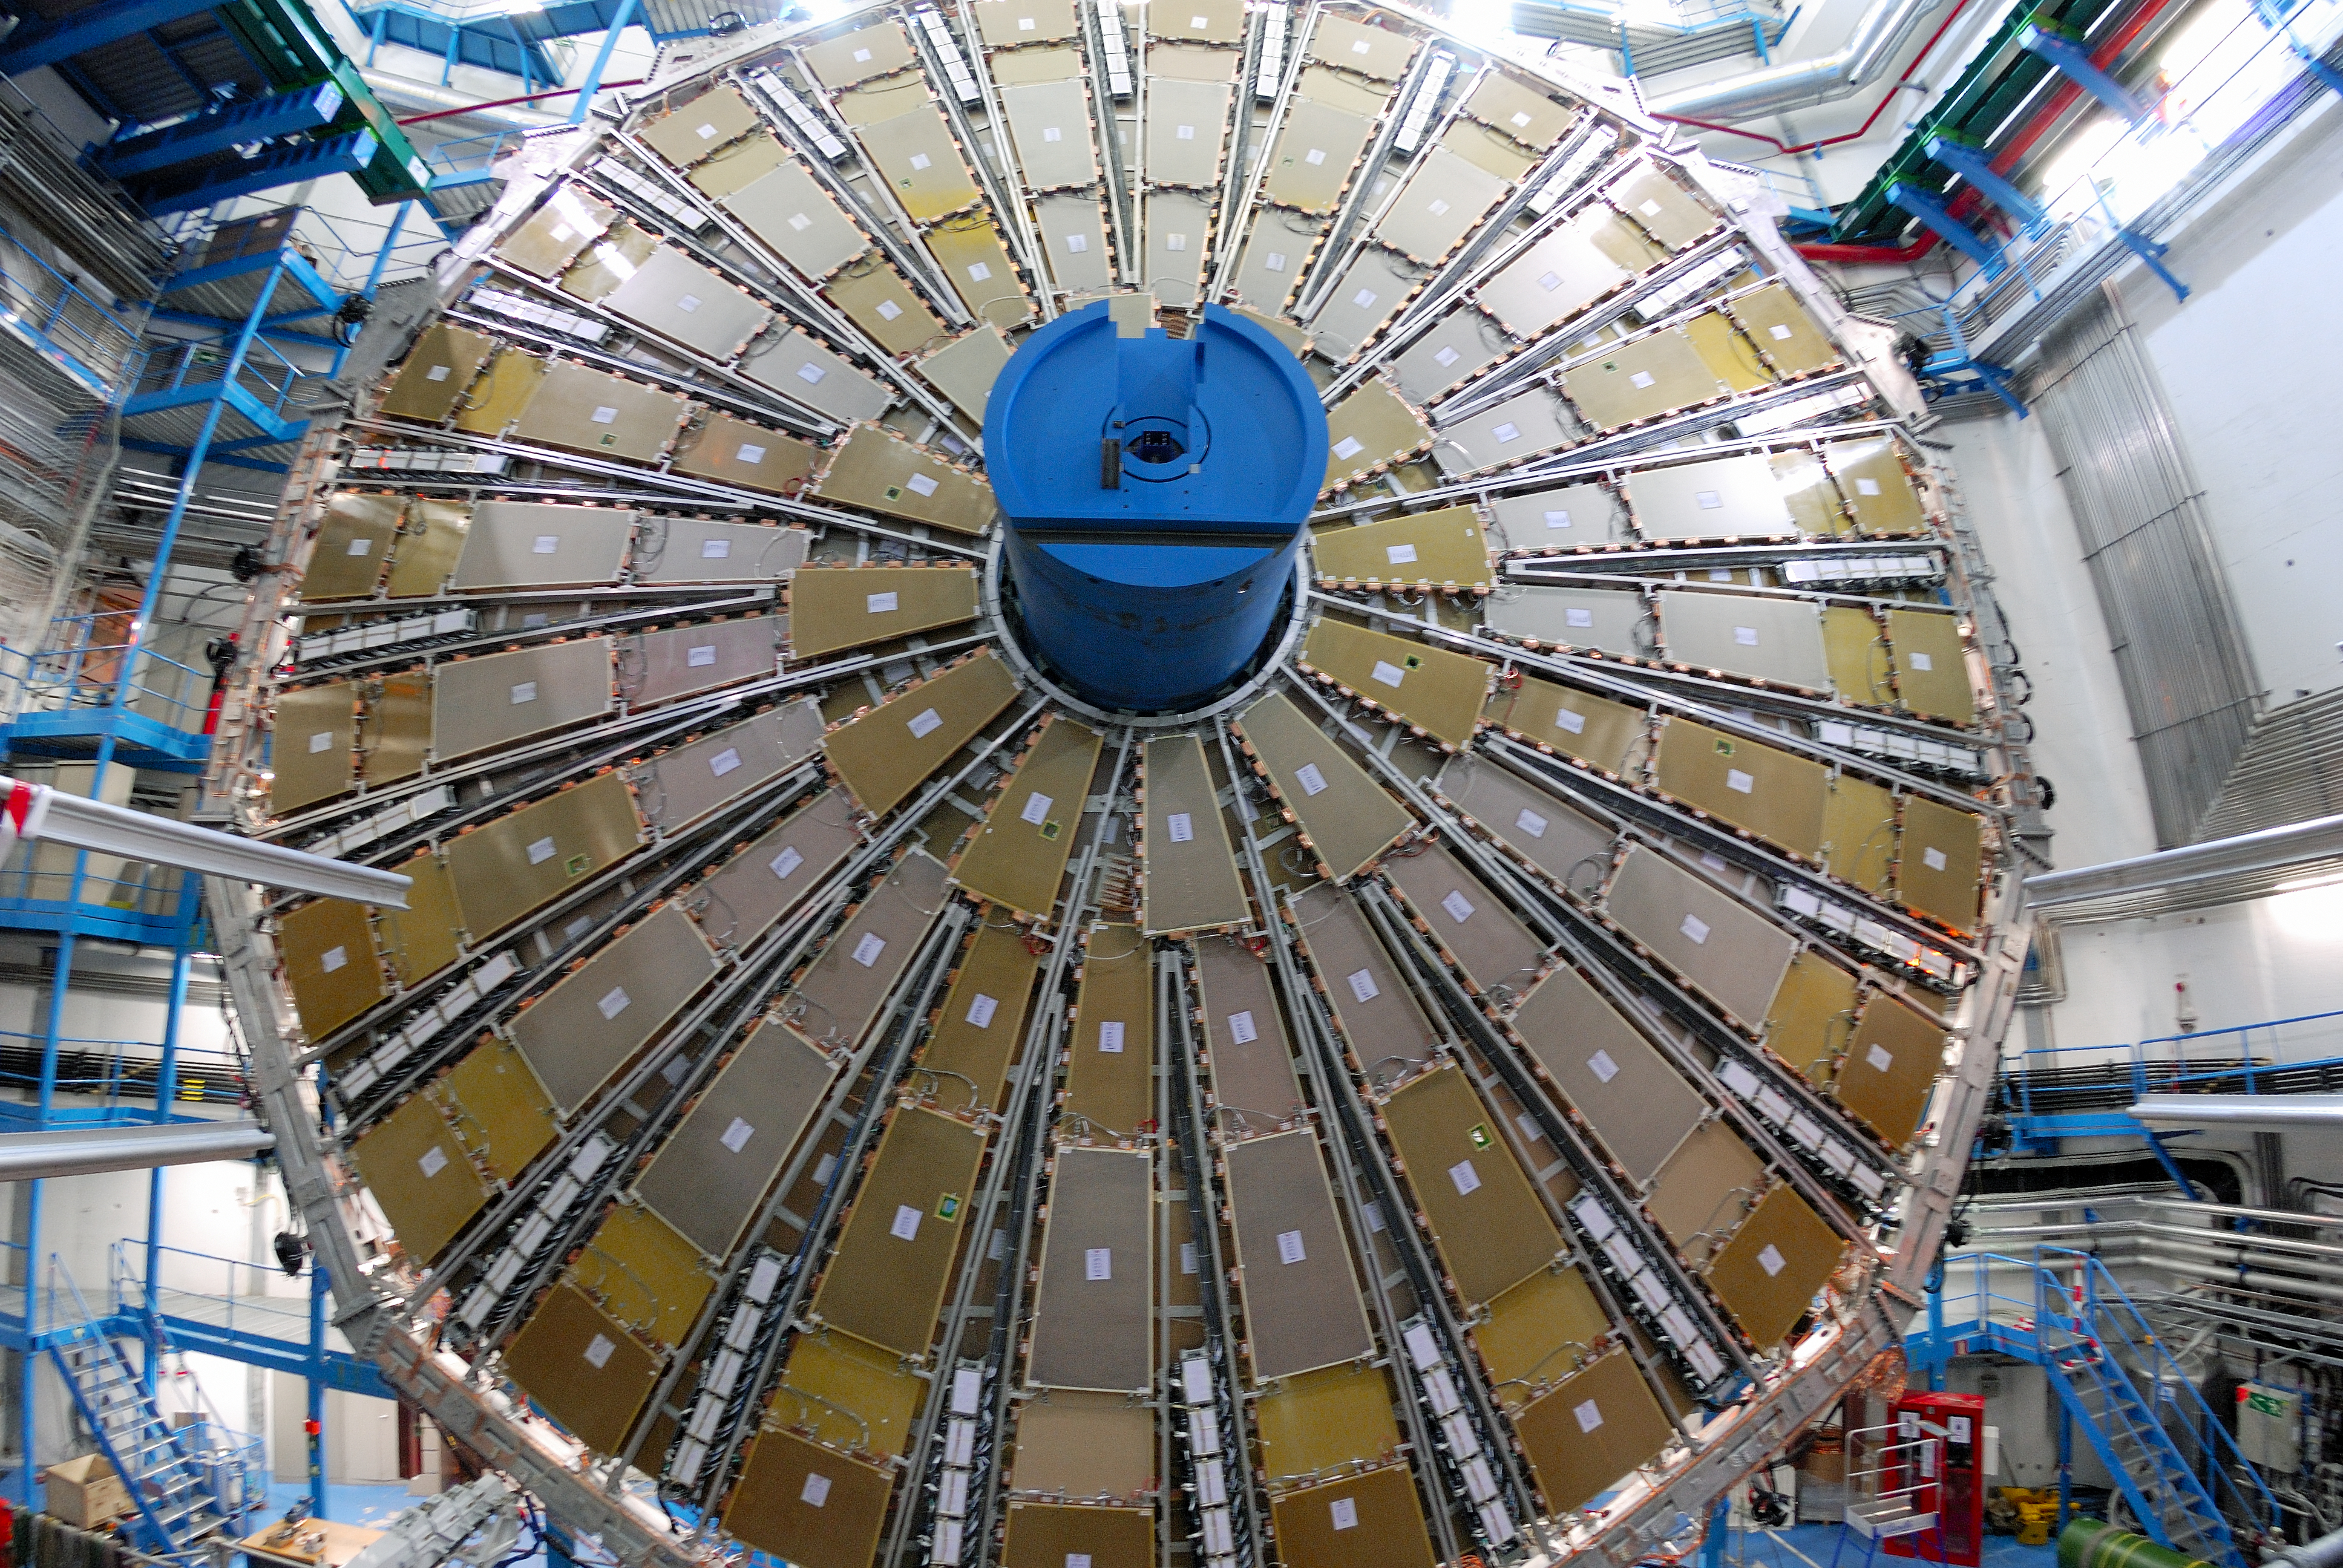
\includegraphics[width=0.95\textwidth]{figs/chapter2/TGC_pic.jpg}
  \caption{The picture of one side of TGC BW, including 24 sectors along $\phi$ direction.\cite{TGCInstallation}.}
  \label{fig:TGC_pic}
\end{figure}

TGCs are multi-wire proportional chambers (MWPCs), as illustrated in Figure~\ref{fig:TGC_cross_section}. The chamber contains \textit{wires} and \textit{strips}, which are arranged orthogonally to enable a two-dimensional readout. As the name suggests, the \textit{wire segments}, which include the sense wires, provide measurement in $R$ direction, while the \textit{strip segments} correspond to the $\phi$ direction. The chambers are filled with a gas mixture of CO$_2$ and n-C$_5$H$_{12}$, with a high voltage of 2.8~kV applied to the wires. To achieve a high time resolution for bunch crossing identification, the interval between sense wires is designed to be 1.8~mm in order to reduce drift time and signal readout delay.

\begin{figure}[htbp]
  \centering
  \includegraphics[width=0.7\textwidth]{figs/chapter2/TGC_cross_section.png}
  \caption{The structure of TGC, including anode wires, graphite cathodes, G-10 layers and a pick-up strip, orthogonal to the wires.\cite{ATLASDetector2008}.}
  \label{fig:TGC_cross_section}
\end{figure}

For higher space resolution during reconstruction, stations are composed of multiple layers. The M1 station contains three layers of wires and two layers of strips (\textit{triplet}), while M2 and M3 consist of two layers each for both wires and strips (\textit{doublet}). The wire and strip signals are read out by grouping them. These readout channels of wires and strips from these doublet or triplet layers are all ``staggered'' intentionally with adjacent layers, generating the conception of \textit{staggered ID}. Each staggered ID corresponds to a unique channel combination that spans across offset wire or strip layers, and enables finer position resolution. In M1 with three wire layers staggered by 1/3 each, the staggered ID achieves roughly 1/3 of the layer's intrinsic spatial resolution. In M2 and M3, the two-layer structure results in a resolution gain of roughly 1/2 per ID unit. The staggered IDs are systematically defined and registered in databases, allowing consistent identification across layers during pattern recognition and offline reconstruction. 

\begin{comment}
\begin{figure}[htbp]
  \centering
  \includegraphics[width=0.95\textwidth]{figs/chapter2/staggeredID_small.png}
  \caption{A part of correspondence table of endcap wire segment between channel number and staggered ID.}
  \label{fig:staggeredID}
\end{figure}
\end{comment}
%====================================================================================================
\subsection{New Small Wheel (NSW)}
%====================================================================================================
The New Small Wheel (NSW) is a muon detector located inside the toroidal magnetic field region, covering the pseudorapidity range of $1.3 < |\eta| < 2.7$. In order to deal with the degradation in tracking efficiency and momentum resolution for muons~\cite{Muon_TDR_NSW}, the NSW replaces the former Cathode Strip Chambers (CSCs) and the inner Multi-Wire Drift Tubes (MDTs) used until LS2 in the endcap region. The NSW has two sides, each consisting of 16 sectors, including 8 large sectors and 8 small sectors overlapping each other in terms of angular coverage. The illustration of NSW sectors layout and the layer structure are shown in Figure~\ref{fig:NSW}. The NSW consists of 16 layers arranged in a sandwiched structure: four layers of small-strip Thin Gap Chambers (sTGCs), followed by two sets of four-layer Micromegas (MM) chambers, and again four layers of sTGCs. This multilayer configuration enables precise determination of muon position and angle based on the combination of hit positions across layers.

\begin{figure}[htbp]
  \centering
  \includegraphics[width=0.95\textwidth]{figs/chapter2/NSW.png}
  \caption{Schematic of the NSW layout and layer structure \cite{ATLASRun3Detector}.}
  \label{fig:NSW}
\end{figure}

The sTGC, short for ``Small-strip Thin Gap Chamber'', is named after its much finer strip pitch compared to the TGC chambers introduced above. It consists of a grid of 50~µm gold-plated tungsten wires arranged with a 1.8~mm pitch, sandwiched between two cathode planes positioned 1.4~mm from the wire plane. The MM is a micro-pattern gaseous detector composed of a 5~mm drift gap and a 128~$\mu$m amplification region separated by a stainless-steel mesh. The amplified signals are read out via 400~$\mu$m pitch strips. The NSW is designed to achieve spatial resolutions of 0.005 in $\eta$, 10~mrad in $\phi$, and an angular resolution of 1~mrad relative to the beam axis.

During Run~3, the NSW, together with the Tile Calorimeter and outer TGC detectors, participates in ``Inner Coincidence'' logic of the endcap muon trigger to reject ``fake muons'' not originating from the interaction point (IP). For the HL-LHC upgrade, additional detectors such as TGC EIL4 and RPC BIS78 will be introduced for the endcap muon trigger system to support this coincidence scheme, further reducing the trigger rate and improving efficiency. Figure~\ref{fig:InnerCoin} demonstrates the inner coincidence logic by showing an example of fake muon in HL-LHC.

\begin{figure}[htbp]
  \centering
  \includegraphics[width=0.95\textwidth]{figs/chapter2/InnerCoin_new2.png}
  \caption{An example of a ``fake muon'', which is a charge particle initially originated from the beam pipe rather than the IP \cite{InnerCoinPoster}.}
  \label{fig:InnerCoin}
\end{figure}

%====================================================================================================
\section{TDAQ System} \label{sec:TDAQSystem}
%====================================================================================================
In the ATLAS experiment, the selection and recording of events is handled by the Trigger and Data Acquisition (TDAQ) system, consisting of the Trigger System and the Data Acquisition System. They are introduced as below.
%====================================================================================================
\subsection{Trigger System}
%====================================================================================================
The proton-proton collisions occurring at a frequency of 40~MHz at the LHC, resulting in a total inelastic interaction rate of about 2~GHz in Run~3. Therefore, it is unpractical to record all the events from proton-proton collisions. In addition to the massive data volume, the vast majority of collision events are dominated by interactions with particles with only small $p_{\mathrm{T}}$, regarded as background that do not arouse interests. To address this, ATLAS employs a trigger system to select events of potential interest only for further physics analysis.

The trigger system is divided into two sequential stages: a hardware-based Level-1 Trigger (L1 Trigger) that performs a fast initial selection, and a software-based High-Level Trigger (HLT) that provides a further event selection with higher precision as the second step in Run~3. A schematic of ATLAS trigger system in Run~3 is shown in Figure~\ref{fig:trigger_run3}.

The L1 trigger primarily receives inputs from two independent systems: \textit{L1Muon} and \textit{L1Calo}, which use custom electronics to trigger on reduced-granularity information from the muon detectors and calorimeters, respectively. A third component, the \textit{L1Topo} processor, applies real-time topological selection criteria based on kinematic informations in the L1Muon and L1Calo systems. The trigger decision at L1 is made by the Central Trigger Processor (CTP), which receives input from L1Muon via the Muon-to-Central Trigger Processor Interface (MUCTPI), from L1Calo, L1Topo, and other auxiliary subsystems. Up to 512 different L1 trigger items can be configured in the CTP. The L1 system reduces the event rate from 40~MHz to a maximum of 100~kHz within a latency constraint of less than 2.5~$\mu$s. 

Once the events are accepted at L1 trigger, they are then sent to a software-based HLT. At this stage, \textit{online} reconstruction algorithms analyze the data at progressively higher levels within restricted Regions-of-Interest (RoIs) identified by L1. These algorithms apply more detailed and computationally intensive reconstruction and selection criteria. The HLT software is incorporated in the ATLAS software framework, Athena, which is also used in \textit{offline} analysis for recorded data. This Athena framework is introduced in Chapter~\ref{ch:Athena}. After HLT processing, the final data output rate is reduced to approximately 3~kHz for Run~3, which will then be written to permanent storage for analysis.

\begin{figure}[htbp]
  \centering
  \includegraphics[width=1.0\textwidth]{figs/chapter2/trigger_run3_1.png}
  \caption{Schematic overview of the ATLAS trigger system in Run~3, showing the two-tier architecture of L1 and HLT triggers \cite{ATLASRun3Trigger}.}
  \label{fig:trigger_run3}
\end{figure}

%====================================================================================================
\subsection{Data Acquisition System}
%====================================================================================================
The Data Acquisition (DAQ) system is responsible for the transport and assembly of data cooperating with the two-level trigger system. It begins at the detector-specific front-end and off-detector electronics, which perform series of data processing and monitoring features before passing the trigger and other downstream systems. In Run~1 and Run~2 of the LHC, data from the Front-End Electronics (FE) were accepted according to the Level-1 accept (L1A) signal and then transmitted to the Read-Out Drivers (RODs), which subsequently forwarded the accepted data to the common stage Read-Out System (ROS). The ROS, composed of commodity servers equipped with custom-built I/O cards, temporarily stores subdetector data in internal memory buffers, named Read-Out Buffers (ROBs). Data flow from the ROS to the High-Level Trigger (HLT) is orchestrated by the Data Collection Manager (DCM), which handles on-demand data requests from HLT processing nodes (HLTMPPUs). These nodes perform event reconstruction and selection, determining whether events are saved for permanent storage or discarded, and then send this decision to HLT. 

The upgrades for DAQ system in Run~3 are achieved by new modules of the Front-End Link eXchange (FELIX) read-out system and software, running on commodity servers (SW ROD), which are integrated into the read-out path for detector systems with upgraded electronics. L1 Calo, L1 Muon and the Central Trigger all send accepted data to the Read-Out System (or FELIX/Software ROD). Both ROS and SW ROD interfaces present a unified interface to the HLT, enabling data routing in both scenarios. Once the HLT processing has been completed, passed events are forwarded to a dedicated cluster of servers (known as Sub-Farm Outputs (SFOs)) for processes like packing, compression, and transfer to offline storage. The bandwidth to permanent storage in Run~3 are allowed for up to 8 GB/s \cite{ATLASRun3Trigger}.

%====================================================================================================
\section{Upgrade for TDAQ System} \label{sec:TDAQUpgrade}
%====================================================================================================
To cope with the significantly increased event rates at the HL-LHC, the ATLAS TDAQ system is undergoing a comprehensive Phase-II upgrade. The upgraded baseline design is shown schematically in Figure~\ref{fig:TDAQ_baseline}. which includes enhancements to the Level-0 (L0) Trigger, Event Filter (EF) and Data Acquisition (DAQ) systems.

The upgraded Level-0 Trigger System consists of subsystems of L0Calo, L0Muon, the Global Trigger, and the Central Trigger Processor (CTP). The L0Calo system is mainly based on the former L1Calo system with minor changes. For L0Muon, a thorough upgrade is performed comparing to Run~3, allowing it identify muon candidates by data from all the muon subsystems and a subset of the Tile Calorimeter. To improve the trigger coverage, new RPC inner stations and new function of MDT precise momentum measurements are added into L0Muon system. The Global Trigger system are implemented newly as a subsystem of L0 Trigger, which is responsible for offline-like algorithms on full-granularity calorimeter data. The event rate after L0 Trigger filtering will be less than 1~MHz.

Once the accept signal from the Level-0 trigger (L0A) is issued, event data from detector front-end electronics are sent to the FELIX system, as the first component of the Readout subsystem. From there, data are routed through the Data Handlers and buffered in the Dataflow subsystem. The Dataflow subsystem ``adjust'' the event data by a series of processes like buffering, transporting, aggregating and compressing, to ensure consistency with the input interface of the Event Filter (EF) system.

The Event Filter (EF) system is based on the Processor Farm \cite{TDAQ_TDR_EF}, a heterogeneous system consisting of CPU cores and accelerators, to perform the EF reconstruction which includes the compute intensive ITk track reconstruction. By a series of processes, events accepted by the EF are eventually reduced to a rate of 10~kHz. The raw output event size is about 6~MB, and the total bandwidth is 60~GB/s.

\begin{figure}[htbp]
  \centering
  \includegraphics[width=1.0\textwidth]{figs/chapter2/TDAQ_baseline_new.png}
  \caption{Baseline design of the upgraded TDAQ system for HL-LHC \cite{TDAQ_TDR_EF}.}
  \label{fig:TDAQ_baseline}
\end{figure}

%====================================================================================================
\section{Upgrade for Muon Trigger System} \label{sec:MuonTriggerUpgrade}
%====================================================================================================
The upgraded Level-0 Muon Trigger System for the HL-LHC is expected to deal with higher trigger rates and improve muon trigger efficiency. The upgrade strategy is illustrated as a block diagram in Figure~\ref{fig:muon_trigger_upgrade}. It consists of several main components: the Barrel Sector Logic, Endcap Sector Logic, the NSW Trigger Processor, and the MDT Trigger Processor. Both the Sector Logic and the NSW Trigger Processor components installed during LS2 will be replaced with new hardware to accommodate the higher performance requirements. The Barrel Sector Logic receives hit information from the RPC and energy flags from the Tile Calorimeter. The Endcap Sector Logic, covering the region $1.05 < |\eta| < 1.3$, receives hits from TGC and RPC. At $1.3 < |\eta| < 2.4$, muon trigger rates are reduced by TGC and NSW, retaining the efficiency for the muons with the transverse momentum $p_\mathrm{T}$ higher than the threshold. The NSW Trigger Processor will be deployed as a separate component from Sector Logic due to large amount of resources consumed by track-segment reconstruction of NSW hits. After initial candidate track reconstruction, the Sector Logic sends these candidates to the newly added MDT Trigger Processor, which offers higher spatial resolution than TGC and RPC, for a refined $p_\mathrm{T}$ estimation. The filtered candidates are then passed back to the Sector Logic, and the final muon trigger decisions are forwarded to Level-0 MUCTPI.

\begin{figure}[htbp]
  \centering
  \includegraphics[width=1.0\textwidth]{figs/chapter2/muon_trigger_upgrade.png}
  \caption{Block diagram of the upgrade strategy of Level-0 muon trigger system at HL-LHC \cite{TDAQ_TDR}.}
  \label{fig:muon_trigger_upgrade}
\end{figure}
